\documentclass{article}

% --- Required Packages ---
\usepackage[a4paper, margin=0in]{geometry}
\usepackage{fontspec}
\usepackage[svgnames]{xcolor}
\usepackage{graphicx}
\usepackage{tikz}
\usetikzlibrary{positioning}
\usepackage{hyperref}
\hypersetup{
    colorlinks=true,
    linkcolor=blue,
    filecolor=magenta,      
    urlcolor=cyan,
    pdftitle={Krider's Field Guide}, % Corrected document title
    pdfpagemode=FullScreen,
    }

% --- COLOR PALETTE ---
\definecolor{PaperColor}{HTML}{FDF5E6}
\definecolor{TextColor}{HTML}{36454F}
\definecolor{KriderYellow}{HTML}{FDF5E6}
\definecolor{KriderGreen}{HTML}{5E7756}
\definecolor{KriderDarkText}{HTML}{36454F}

% --- Document-wide Settings ---
\setmainfont{Roboto}[
    UprightFont = *,
    BoldFont = * Bold,
    ItalicFont = * Italic
]
\pagenumbering{gobble}

% --- Document Body ---
\begin{document}
\pagestyle{empty}

%---------------------------------------------------
% PAGE 1: Krider's Field Guide Cover (Corrected Layout)
%---------------------------------------------------
\begin{tikzpicture}[remember picture, overlay]
    \coordinate (C) at (current page.center);

    % --- Background ---
    \fill[KriderYellow] (current page.south west) rectangle (current page.south east);

    % --- Header Block ---
    \node[KriderDarkText, anchor=north west, align=left] at (current page.north west) [xshift=1.5cm, yshift=-1.5cm] {
        \normalfont \fontsize{10}{12}\selectfont Powered by \{data\}syntax
    };
    
    % --- Main Title (Above Image) ---
    \node[KriderDarkText, anchor=center, text centered] at (current page.north) [yshift=-3cm] {
        \bfseries \fontsize{50}{66}\selectfont Krider's  Field Guide
    };
    
    % --- Subheadings ---
    \node[KriderDarkText, anchor=center] at (current page.north) [yshift=-5cm] {
        \normalfont\itshape \fontsize{16}{20}\selectfont Continuing a Legacy of Horticultural Excellence Since 1906 
    };

    % --- Main Image (Resized and placed below the title) ---
    \node[anchor=center] at ([yshift=.8cm]C) {
        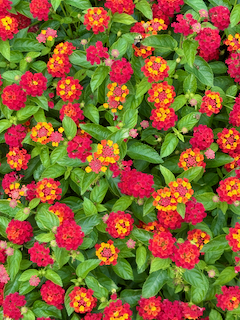
\includegraphics[width=12.5cm]{coverFlower.png}
    };
    
    % --- Bottom Product Box (with green background) ---
    \node[fill=KriderGreen, text=white, anchor=south, minimum width=\paperwidth-2cm, inner sep=15pt, outer sep=0, rounded corners=3pt] at (current page.south) [yshift=3.8cm] {
        \begin{minipage}{0.9\textwidth}
            \bfseries \fontsize{18}{20}\selectfont Lantana (Lantana camara L.) \\[3mm]
            \normalfont \fontsize{14}{15}\selectfont A multi-colored flower clusters that often shift in hue as they mature, the Lantana is a example of nature's artistry. While prized globally as a decorative shrub, it holds a dual identity. Originally native to the American tropics, this plant is also considered one of the world's most invasive species, able to thrive in the most extreme climates. \\
            \\
            Beyond its controversial reputation, the Lantana possesses a complex chemistry that has made it a subject of interest in everything from traditional medicine to modern research into its potential for creating handmade paper and even novel anticancer compounds.

        \end{minipage}
    };
    
    % --- Krider Logo Footer (Bottom Left) ---
    \node[anchor=south west, align=left, text width=4in] at (current page.south west) [xshift=1.5cm, yshift=1.5cm] {
        \bfseries\itshape \fontsize{24}{24}\selectfont Krider's Field Guide \\
        \itshape\bfseries \fontsize{10}{12}\selectfont Week 46 - Fall - 2025 \\
        \normalfont\itshape \fontsize{9}{11}\selectfont Guide: 004
    };
    
    % --- Page Footer ---
    \node[KriderDarkText, anchor=center] at (current page.south) [yshift=20] {
        \fontsize{12}{14}\itshape Page 1 of 3
    };
\end{tikzpicture}

\newpage

%---------------------------------------------------
% PAGE 2: Professional 2x2 Rose Grid Page
%---------------------------------------------------
\begin{tikzpicture}[remember picture, overlay]
    \fill[KriderYellow] (current page.south west) rectangle (current page.north east);
    \coordinate (C) at (current page.center);

    % --- Main Title ---
    \node[KriderDarkText, anchor=north, text width=0.9\paperwidth, align=center] at (current page.north) [yshift=-3cm] {
        \bfseries\fontsize{36}{40}\selectfont 
    };

    % --- Define a style for each content block for consistency ---
    \tikzset{rose_block/.style={text width=8cm, align=center}}

    % --- Top Left Flower ---
    \node[rose_block] at ([xshift=-5cm, yshift=6.5cm]C) {
        
\includegraphics[width=7cm]{flower1.png} \\
        \vspace{5mm}
        \bfseries\fontsize{16}{18}\selectfont American Rhododendron \\
        \normalfont\itshape\fontsize{11}{13}\selectfont(Rhododendron maximum L.) \\
    
        
    };

    % --- Top Right Flower ---
    \node[rose_block] at ([xshift=5cm, yshift=7.5cm]C) {
        
\includegraphics[width=7cm]{flower2.png} \\
        \vspace{5mm}
        \bfseries\fontsize{16}{18}\selectfont Higan cherry \\
        \normalfont\itshape\fontsize{11}{13}\selectfont (Prunus × subhirtella Miq) \\
    };

    % --- Bottom Left Flower ---
    \node[rose_block] at ([xshift=-5cm, yshift=-5.5cm]C) {
        
\includegraphics[width=7cm]{flower3.png} \\
        \vspace{5mm}
        \bfseries\fontsize{16}{18}\selectfont Bloodroot \\
        \normalfont\itshape\fontsize{11}{13}\selectfont (Sanguinaria canadensis L.) \\
    };

    % --- Bottom Right Flower ---
    \node[rose_block] at ([xshift=5cm, yshift=-5.5cm]C) {
        
\includegraphics[width=7cm]{flower4.png} \\
        \vspace{5mm}
        \bfseries\fontsize{16}{18}\selectfont Rose \\
        \normalfont\itshape\fontsize{11}{13}\selectfont (Rosa lucieae Franch. \& Rochebr. ex Crép) \\
    };

    % --- Page Footer ---
    \node[KriderDarkText, anchor=center] at (current page.south) [yshift=50] {
        \fontsize{12}{14}\itshape Page 2 of 3
    };
\end{tikzpicture}

\newpage

%---------------------------------------------------
% PAGE 3: CITATION PAGE (Themed)
%---------------------------------------------------
\begin{tikzpicture}[remember picture, overlay]
    \fill[KriderYellow] (current page.south west) rectangle (current page.north east);
    
    % --- Main Title ---
    \node[KriderDarkText, anchor=center] at (current page.center) [yshift=250] {
        \fontsize{32}{36}\bfseries Project Source \& Collaboration
    };
    
    % --- Explanatory Text ---
    \node[KriderDarkText, anchor=north, text width=0.7\paperwidth, align=center] at (current page.center) [yshift=180] {
        \fontsize{14}{22}\selectfont
        This document was written in \LaTeX. The complete source code, image assets, and project history are available on GitHub. Suggestions, and flower requests are welcome!.
    };

    % --- GitHub Logo and Link ---
    \node[anchor=center] at (current page.center) [yshift=-20] {
        \href{https://github.com/Data-Syntax/KridersFieldGuide}{
\includegraphics[height=5cm]{github-mark.png}}
    };
    
    \node[KriderDarkText, anchor=center] at (current page.center) [yshift=-100] {
        \fontsize{14}{18}\selectfont\url{https://github.com/Data-Syntax/KridersFieldGuide}
    };
    
    % --- Page Footer ---
    \node[KriderDarkText, anchor=center] at (current page.south) [yshift=50] {
        \fontsize{12}{14}\itshape Page 3 of 3
    };
\end{tikzpicture}

\end{document}